% PROSZĘ KOMPILOWAĆ TEN DOKUMENT ZA POMOCĄ SILNIKA XELATEX
% W PRZECIWNYM RAZIE NALEŻY USUNĄĆ PAKIET fontspec ORAZ USTAWIENIA FONTU
% Z PLIKU styles/prez_wmini_pl.sty (PIERWSZE TRZY LINIJKI)
% W PRZYPADKU BRAKU FONTU Adagio Slab NALEŻY ZGŁOSIĆ SIĘ DO BIP PW O JEGO UDOSTĘPNIENIE,
% ZAŁADOWAĆ INNY KRÓJ CZCIONKI LUB ZAKOMENTOWAĆ/USUNĄĆ USTAWIENIA FONTU

\documentclass[aspectratio=169]{beamer}

\usepackage{styles/prez_wmini_pl}
\usepackage{booktabs}
\setbeamertemplate{section in toc}[sections numbered]
\setbeamertemplate{subsection in toc}[subsections numbered]
\usepackage{times}
\usepackage{amsmath}
\usepackage{bm}

\usefonttheme[onlymath]{serif}

\definecolor{quotationcolour}{HTML}{F0F0F0}
\definecolor{quotationmarkcolour}{HTML}{1F3F81}

% Double-line for start and end of epigraph.
\newcommand{\epiline}{\hrule \vskip -.2em \hrule}
% Massively humongous opening quotation mark.
\newcommand{\hugequote}{%
  \fontsize{42}{48}\selectfont \color{quotationmarkcolour} \textbf{``}
  \vskip -.5em
}

% Beautify quotations.
\newcommand{\epigraph}[2]{%
  \bigskip
  \begin{center}
  \colorbox{quotationcolour}{%
    \parbox{.80\textwidth}{%
    \epiline \vskip 1em {\hugequote} \vskip -.5em
    \parindent 2.2em
    #1\vspace{-.25cm}\begin{flushright}\textsc{#2}\end{flushright}
    \epiline
    }
  }
  \end{center}
  \bigskip
}

\graphicspath{ {./images/} }



% ------------------ Ustawienia użytkownika ------------------
% kolor tytułu prezentacji; zalecany white lub grafitowy.
% Poza tym można użyć zdefiniowanych w pakiecie kolorów:
% sloneczny, morelowy, mietowy, mokka, grafitowy, sliwkowy, szafirowy, wrzosowy
% lub wybrać sobie kolor z pakietu xcolor
\colorlet{title_color}{grafitowy}

\title{Opracowanie wirtualnego środowiska\\do symulacji dynamiki lotu\\ bezzałogowych statków powietrznych}
%\subtitle{Podtytuł consectetur adispiscing elit}
\author{Wojciech Gajda \and  Igor Faliszewski}
\date{28 listopada 2023} % można tam wpisać datę jaką się chce lub zakomentować dla daty dzisiejszej



% ------------------ Początek prezentacji ------------------

\begin{document}
\sloppy

% Slajd tytułowy
{
\maketitleframe 
}

\begin{frame}
\frametitle{Agenda}
  \tableofcontents[  
    sectionstyle=show, 
    %hideallsubsections
    ]
\end{frame}

\section{Wprowadzenie}
\subsection{Motywacje}
\begin{frame}%[allowframebreaks]
	\frametitle{Motywacja}
	\begin{columns}
		\begin{column}{0.33\textwidth}
	   	 	\begin{figure}
	   		 \centering
	      		 \uncover<2->{
\includegraphics[width=0.9\textwidth]{logos/warthunder.png}}
	    		\end{figure}
	    		\begin{figure}
	   		 \centering
	      		 \uncover<3->{
\includegraphics[width=0.9\textwidth]{logos/MFS.png}}
	    		\end{figure}
		\end{column}
		\begin{column}{0.33\textwidth}
	   	 	\begin{figure}
	   		 \centering
	      		 \uncover<4->{
\includegraphics[width=0.9\textwidth]{logos/ardupilot.jpg}}
	    		\end{figure}
	    		\begin{figure}
	   		 \centering
	      		 \uncover<5->{
\includegraphics[width=0.9\textwidth]{logos/betaflight.png}}
	    		\end{figure}
	    		\begin{figure}
	   		 \centering
	      		 \uncover<6->{
\includegraphics[width=0.9\textwidth]{logos/inav.png}}
	    		\end{figure}
		\end{column}
		\begin{column}{0.33\textwidth}
	    		\begin{figure}
	   		 \centering
	      		 \uncover<7->{
\includegraphics[width=0.5\textwidth]{logos/JSBSim.png}}
	    		\end{figure}
			\begin{figure}
	   		 \centering
	      		 \uncover<8->{
\includegraphics[width=0.5\textwidth]{logos/VBS.png}}
	    		\end{figure}
		\end{column}
	\end{columns}
\end{frame}

\begin{frame}%[allowframebreaks]
	\frametitle{Motywacja}
	\begin{columns}
		\begin{column}{0.33\textwidth}
	   	 	\begin{figure}
	   		 \centering
	      		 \uncover<2->{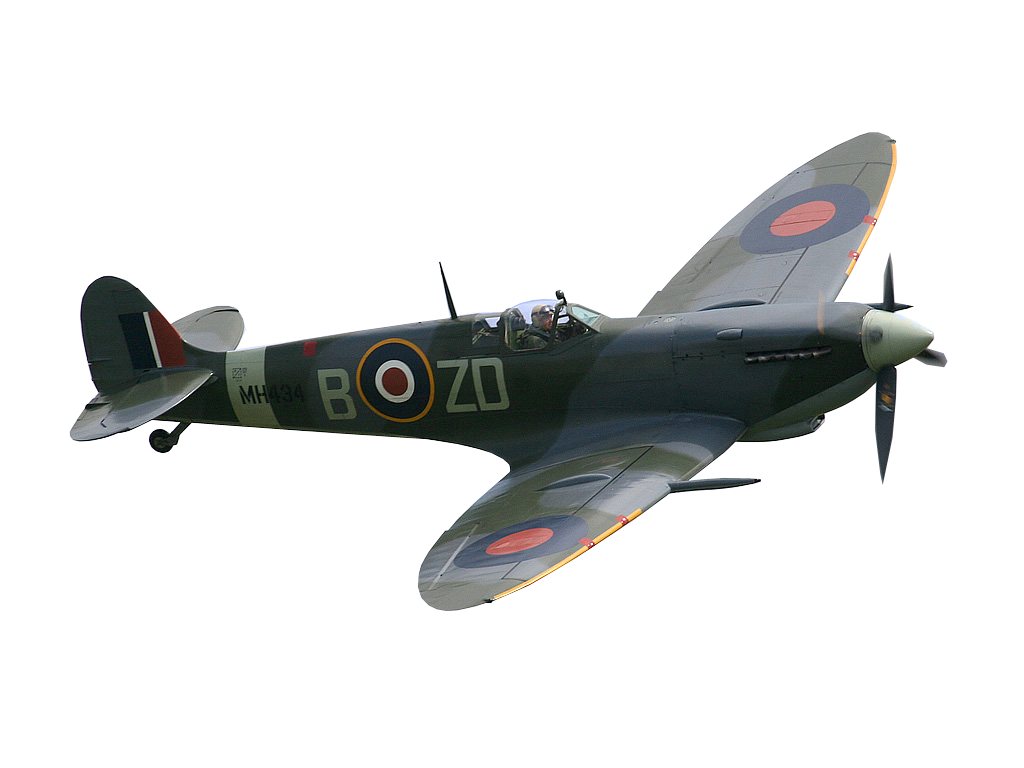
\includegraphics[width=0.9\textwidth]{spitfire.png}}
	    		\end{figure}
		\end{column}
		\begin{column}{0.33\textwidth}
	   	 	\begin{figure}
	   		 \centering
	      		 \uncover<3->{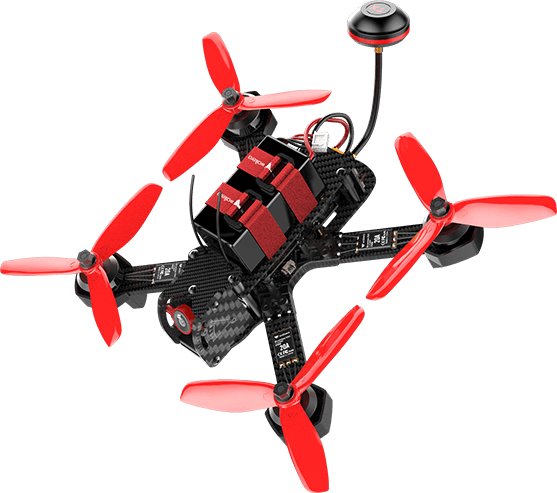
\includegraphics[width=0.9\textwidth]{quadcopter_fpv.png}}
	    		\end{figure}
		\end{column}
		\begin{column}{0.33\textwidth}
	    		\begin{figure}
	   		 \centering
	      		 \uncover<4->{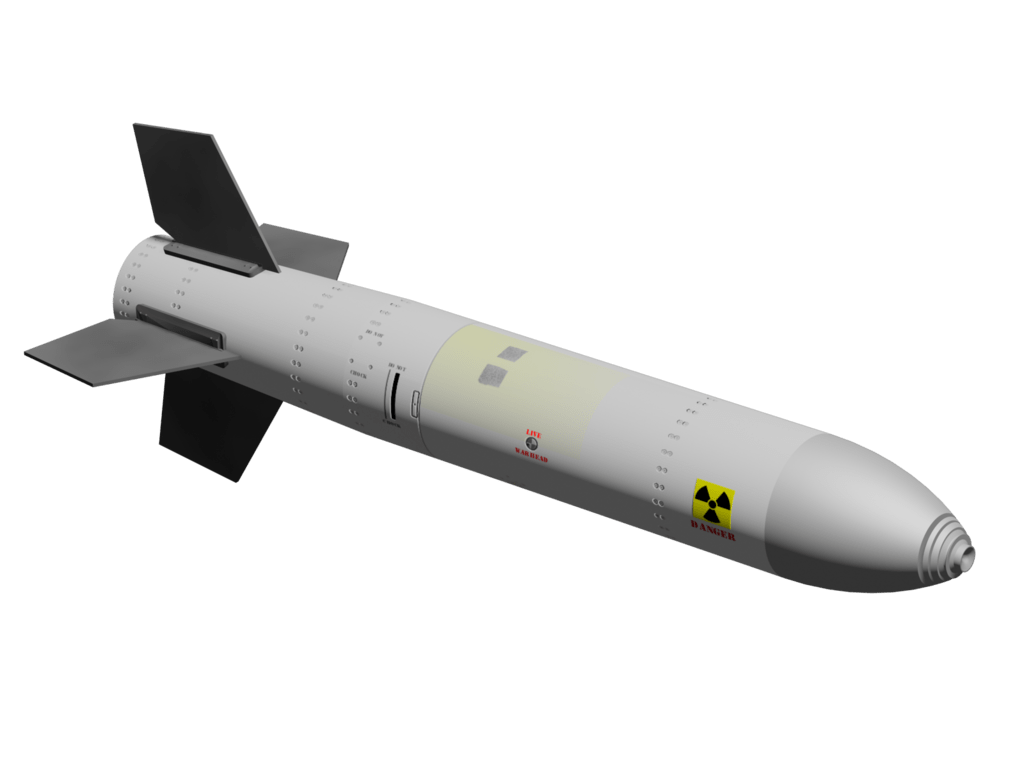
\includegraphics[width=0.9\textwidth]{missile.png}}
	    		\end{figure}
		\end{column}
	\end{columns}
	\begin{figure}
		\hfill
		\uncover<5->{
\includegraphics[width=0.2\textwidth]{helicopter_ban.png}}
	\end{figure}
\end{frame}

\subsection{Cel projektu}
\begin{frame}%[allowframebreaks]
	\frametitle{Cel projektu}
	  \begin{itemize}
	  \item {
	    First item.
	    \pause % Tu nastąpi pauza
	  }
	  \item {   
	    Second item.
	  }
	  % Można ustalić kiedy dany element ma się pojawić, używając <n->:
	  \item<3-> {
	    Third item.
	  }
	  \item<4-> {
	    Fourth item.
	  }
	  % można użyć komendy \uncover żeby ,,odkryć'' cokolwiek, nie tylko item
	  \item<5-> {
	    Fifth item. \uncover<6->{Extra text in the fifth item.}
	  }
 	 \end{itemize}
\end{frame}

\section{Wstep teoretyczny}
\begin{frame}%[allowframebreaks]
	\frametitle{Wstep teoretyczny}
	 \uncover<2->{\epigraph{There is nothing so practical as a good theory.}{Lewin Kurt}}
	 \uncover<3->{\epigraph{Nie ma osobnej ani teorii, ani praktyki inżynierskiej, jest tylko wspólna sztuka inżynierska.}{prof. Jan Oderfeld}}
\end{frame}


\subsection{Dynamika statku powietrznego}
\begin{frame}%[allowframebreaks]
	\frametitle{Dynamika lotu}
	\begin{columns}
		\begin{column}{0.55\textwidth}
	   	 	\begin{figure}
	   		 \centering
	      		 \uncover<2->{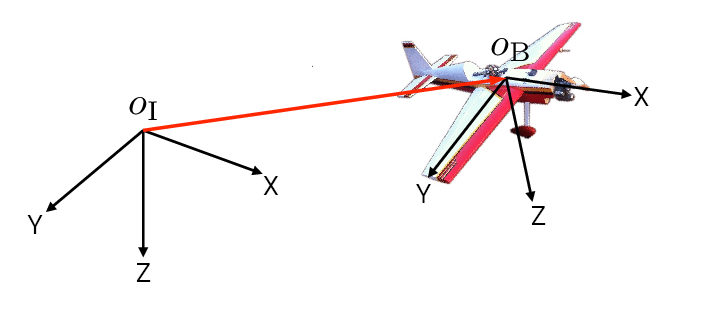
\includegraphics[width=1.05\textwidth]{frames.png}}
	    		\end{figure}
		\end{column}
		\begin{column}{0.45\textwidth}
	   	 	\begin{figure}
	   		 \centering
	      		 \uncover<3->{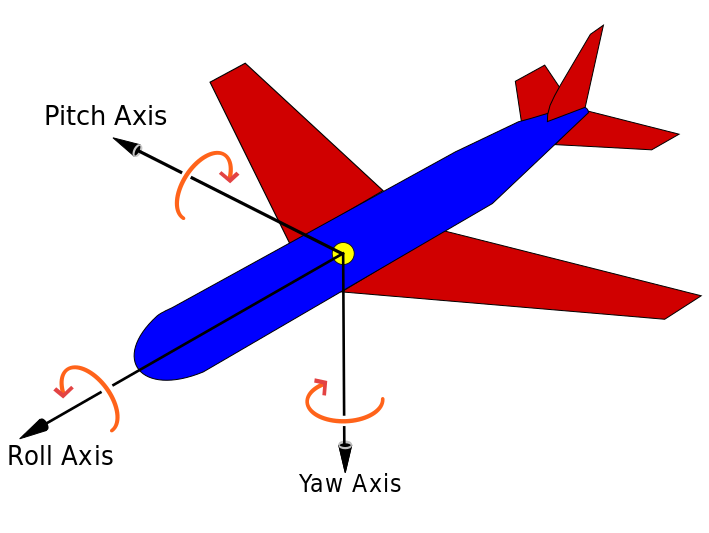
\includegraphics[width=1.05\textwidth]{RPY.png}}
	    		\end{figure}
		\end{column}
	\end{columns}
\end{frame}

\begin{frame}%[allowframebreaks]
	\frametitle{Równania stanu}
	\begin{columns}
		\begin{column}{0.3\textwidth}
	      		 	\uncover<1->{\[
				\begin{cases}
					\dot{\bm{x}} \left(t\right)  = \bm{Ax} \left(t\right)  + \bm{Bu} \left(t\right) \\
					\bm{y} \left(t\right) = \bm{Cx} \left(t\right) + \bm{Du} \left(t\right)
				\end{cases}
				\]}	
	      		 	\[
				\begin{cases}
					\dot{\bm{x}} \left(t\right)  = \bm{f} \left(t,\bm{x}\left(t\right),\bm{u}\left(t\right) \right) \\
					\bm{y} \left(t\right) = \bm{g} \left(t,\bm{x}\left(t\right),\bm{u}\left(t\right) \right)
				\end{cases}
				\]	
		\end{column}
		\begin{column}{0.7\textwidth}
	   	 	\begin{figure}
	   		 \centering
	      		 \uncover<2->{\includegraphics[width=0.9\textwidth]{state\_eq.png}}
	    		\end{figure}
		\end{column}
	\end{columns}
\end{frame}

\begin{frame}%[allowframebreaks]
	\frametitle{Równania różniczkowe}
	\begin{itemize}
	  \item{
	    Przed zastosowaniem algorytmu obniżyć rząd równania różniczkowego.
	    \pause
	  }
	  \item {   
	    Skorzystać z algorytmu jawnego lub niejawnego algorytmu całkowania RR
	    \pause
	  }
	  % Można ustalić kiedy dany element ma się pojawić, używając <n->:
	  \item {
	    Algorytmy jawne:
	    \pause
	    \begin{itemize}
		  \item{
		    Euler: $\bm{x}\left(t + \Delta t\right) = \bm{x}\left(t\right) + \Delta t \cdot \bm{\dot{x}} $
		    \pause
		  }
		  \item {   
		    Rugge-Kutty 4 rzędu
		  }
	     \end{itemize}
	  }
 	 \end{itemize}
\end{frame}

\begin{frame}[allowframebreaks]
	\frametitle{Model matematyczny statku powietrznego}
	
\end{frame}

\begin{frame}[allowframebreaks]
	\frametitle{Kolizje}
	
\end{frame}

\begin{frame}%[allowframebreaks]
	\frametitle{Odrzut}
	\uncover<2->{Zasada zachowania pędu $\vec{\bm{p}}$ i zasada zachowania momentu pędu (krętu) $\vec{\bm{L}}$}.
	\uncover<3->{
	\[
		\begin{bmatrix}
		\vec{\bm{p}}_{przed}\\
		\vec{\bm{L}}_{przed}
		\end{bmatrix}
		=
		\begin{bmatrix}
		\vec{\bm{p}}_{po}\\
		\vec{\bm{L}}_{po}
		\end{bmatrix}
		+	
		\begin{bmatrix}
		\vec{\bm{p}}_{pocisku}\\
		\vec{\bm{L}}_{pocisku}
		\end{bmatrix}	
	\]}
	\uncover<4->{
	\[
		\bm{M}
		\begin{bmatrix}
		\vec{\bm{v}}_{przed}\\
		\vec{\bm{\omega}}_{przed}
		\end{bmatrix}
		=
		\bm{M}
		\begin{bmatrix}
		\vec{\bm{v}}_{po}\\
		\vec{\bm{\omega}}_{po}
		\end{bmatrix}
		+
		\begin{bmatrix}
		\vec{\bm{v}}_{pocisku}\\
		\vec{\bm{r}}_{pocisku} \times  \vec{\bm{v}}_{pocisku}
		\end{bmatrix}	
	\]}
	
\end{frame}

\subsection{Sterowanie statkiem powietrznym}

\begin{frame}
	\frametitle{Sterowanie statkiem powietrznym}
	\begin{figure}
	   		 \centering
	      		 \uncover<2->{\includegraphics[width=0.9\textwidth]{uk\_reg.jpg}}
	\end{figure}
\end{frame}
\begin{frame}
	\frametitle{Sterowanie statkiem powietrznym}
	\begin{figure}
	   		 \centering
	      		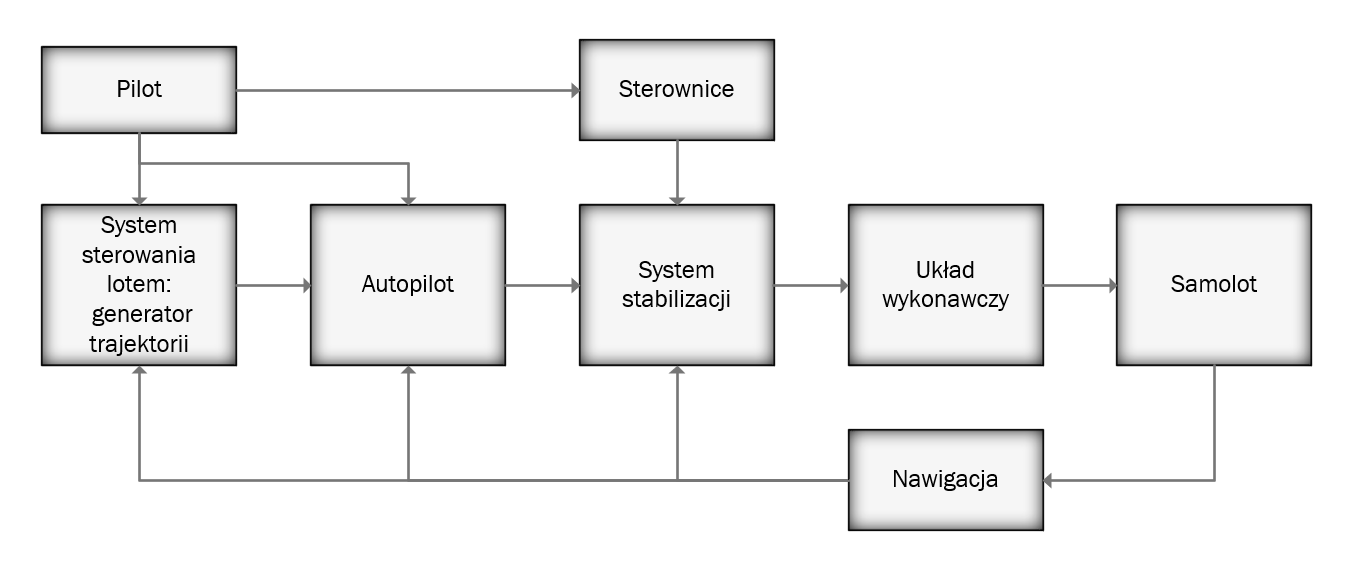
\includegraphics[width=\textwidth]{controller.png}
	\end{figure}
\end{frame}

\begin{frame}%[allowframebreaks]
	\frametitle{Regulator PID}
	\begin{columns}
		\begin{column}{0.5\textwidth}
	   	 	\begin{figure}
	   		 \centering
	      		 \uncover<2->{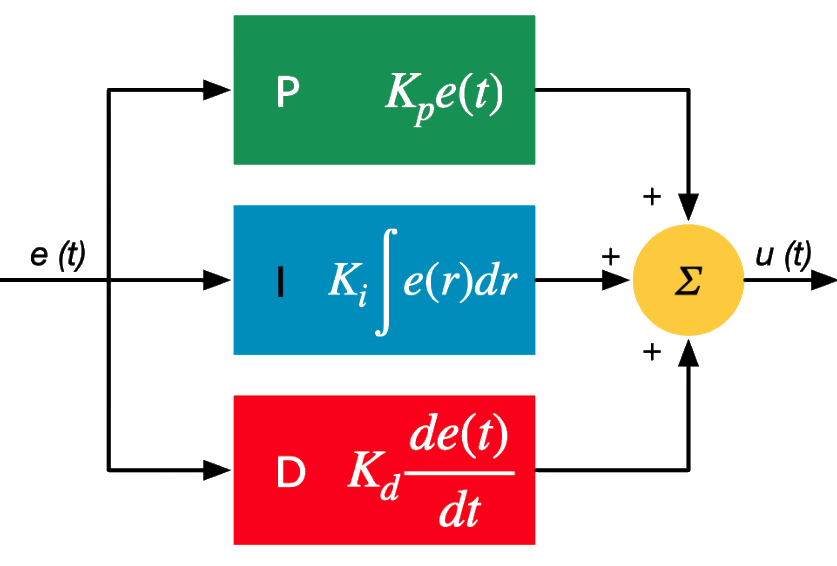
\includegraphics[width=\textwidth]{pid.png}}
	    		\end{figure}
		\end{column}
		\begin{column}{0.5\textwidth}
	   	 	\begin{figure}
	   		 \centering
	      		 \uncover<3->{\includegraphics[width=\textwidth]{pid\_graph.png}}
	    		\end{figure}
		\end{column}
	\end{columns}
	
	
\end{frame}

\begin{frame}
	\frametitle{Sterowanie statkiem powietrznym}
	\begin{figure}
	   		 \centering
	      		 \includegraphics[width=1.05\textwidth]{pid\_cascade.jpg}
	\end{figure}
\end{frame}

\begin{frame}%[allowframebreaks]
	\frametitle{Nawigacja}
	\begin{columns}
		\begin{column}{0.5\textwidth}
	   	 	 Czujniki:
	   	 	 \begin{itemize}
			  \item{
			    Żyroskop
			  }
			  \item {   
			    Akcelerometer
			  }
			  \item {   
			    Barometer
			  }
			  \item {   
			    Czujnik prędkości powietrza
			  }
			  \item {   
			    Nawigacja satelitarna
			  }
			  \item {   
			    Radar, sonar, lidar
			  }
	     \end{itemize}
	     \pause
	   	 	
		\end{column}
		\begin{column}{0.5\textwidth}
			Filtr Kalmana:
	   	 	\begin{figure}
	   		 \centering
	      		 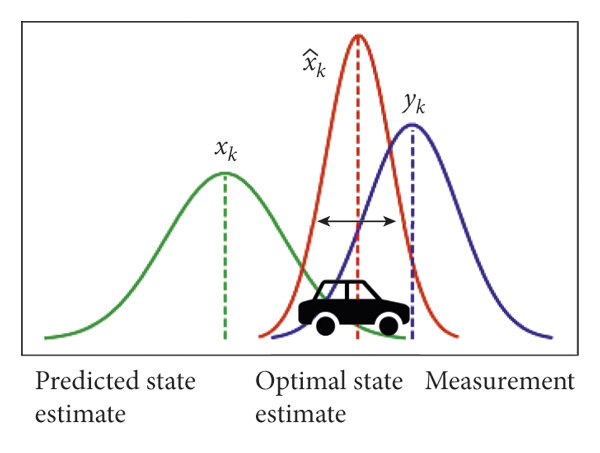
\includegraphics[width=0.8\textwidth]{kalman.png}
	    		\end{figure}
		\end{column}
	\end{columns}
\end{frame}

\subsection{Grafika komputerowa}

\begin{frame}[allowframebreaks]
	\frametitle{Potok renderowania}
	
\end{frame}

\begin{frame}[allowframebreaks]
	\frametitle{Shadery}
	
\end{frame}

\begin{frame}[allowframebreaks]
	\frametitle{GPU}
	
\end{frame}

\begin{frame}[allowframebreaks]
	\frametitle{Cieniowanie i model oświetlenia}
	
\end{frame}

\begin{frame}[allowframebreaks]
	\frametitle{Renderowanie interfejsu}
	
\end{frame}

\begin{frame}[allowframebreaks]
	\frametitle{Obsługa kontrolera}
	
\end{frame}

\begin{frame}[allowframebreaks]
	\frametitle{Krzywa łańcuchowa}
	
\end{frame}

\section{Demo}

\begin{frame}
	  \begin{center}
	\Huge Demo
	\end{center}
\end{frame}


\begin{frame}
	\frametitle{Testy $\alpha$} %JOKE
	\begin{figure}
		\centering
		
\includegraphics[width=0.7\textwidth]{dog.jpg}
	\end{figure}
\end{frame}


\begin{frame}
	\frametitle{Dyskusja}
	\begin{figure}
		\centering
		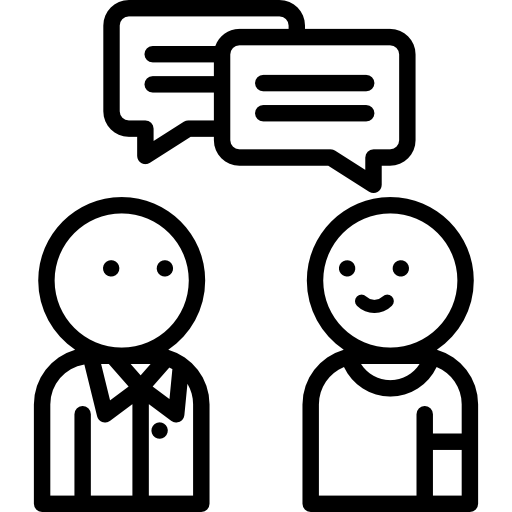
\includegraphics[width=0.7\textwidth]{questions.png}
	\end{figure}
\end{frame}

\begin{frame}{Literatura}
\begin{thebibliography}{10}
\beamertemplatebookbibitems
\bibitem{en15197136}[Energies, 2022] Quadrotor Model for Energy Consumption Analysis
   \newblock  Jacewicz, Mariusz and Żugaj, Marcin and Głębocki, Robert and Bibik, Przemysław

\end{thebibliography}
\end{frame}

\begin{frame}
	  \begin{center}
	\Huge Dziękuje za uwagę!
	\end{center}
\end{frame}

\end{document}